
%%% Local Variables:
%%% mode: latex
%%% TeX-master: "gis18"
%%% End:



\section{Preliminaries}
\label{sec-pre}

In this section, we first introduce some basic concepts for trajectory tracking.
Then we introduce position and trajectory tracking algorithms \ldr and \ldrh that are helpful to understand the basic ideas of the work.
Notations used are summarized in Table \ref{tab:notations}.

\begin{table}
	\renewcommand{\arraystretch}{1.20}
	\caption{\small Summary of notations}
	\vspace{-1.5ex}
	\centering
	\footnotesize
	%\scriptsize
	\begin{tabular}{|c|l|}
		\hline
		{\bf Notations}& {\bf Semantics}   \\		\hline %\hline
		$P$ & a data point \\		\hline
		$\dddot{\mathcal{T}}$ & a trajectory $\dddot{\mathcal{T}}$ is a sequence of data points\\		\hline
		$\overline{\mathcal{T}}$&  {a piece-wise line representation of a trajectory $\dddot{\mathcal{T}}$}	\\		\hline
		$\mathcal{L}$ & a line segment  \\		\hline
		$\epsilon$ & an error bound \\		\hline
		$ped\left(P, \mathcal{L}\right)$ &  {the perpendicular Euclidean distance of point $P$ to line segment $\mathcal{L}$}	\\	\hline
		$sed\left(P, \mathcal{L}\right)$ & {the synchronous Euclidean distance of point $P$ to line segment $\mathcal{L}$} 	\\		\hline
		%$dad\left(\mathcal{L}_1, \mathcal{L}_2\right)$ & {the direction-aware distance of line segment $\mathcal{L}_1$ to line segment $\mathcal{L}_2$} 	%\\		\hline
		\sector{} & a sector \\		\hline
		%		$\overline{A} \times \overline{B}$ & the cross product of (vectors) $\overline{A}$ and $\overline{B}$\\		\hline
		%		$\mathcal{H}(\mathcal{L})$ & The open half-plane to the left of $\mathcal{L}$ \\		\hline
		%		$\mathcal{R}$& a convex polygon \\		\hline
		%		$\mathcal{R}^*$ & the intersection of convex polygons \\		\hline
		%		$m$ & the maximum number of edges of a polygon\\		\hline
		%		$E^j$ & a group of edges labeled with $j$\\		\hline
		%		$g(e)$ & the label of an edge $e$ of polygons \\		\hline
		%		\circle{} & a synchronous circle\\		\hline
		\cone{} & a spatio-temporal cone \\		\hline
		\circle{} & a synchronous circle \\		\hline
		%\pcircle{} & a cone projection circle \\		\hline
		$\mathcal{R}$& a convex polygon \\		\hline
		%$\mathcal{R}^*$ & the intersection of convex polygons \\		\hline
		%$\bigsqcap$ & intersection of geometries\\		\hline
		%$G$ &	the reachability graph of a trajectory\\		\hline
	\end{tabular}
	\label{tab:notations}
	\vspace{-2ex}
\end{table}


\begin{figure}[tb!]
	\centering
	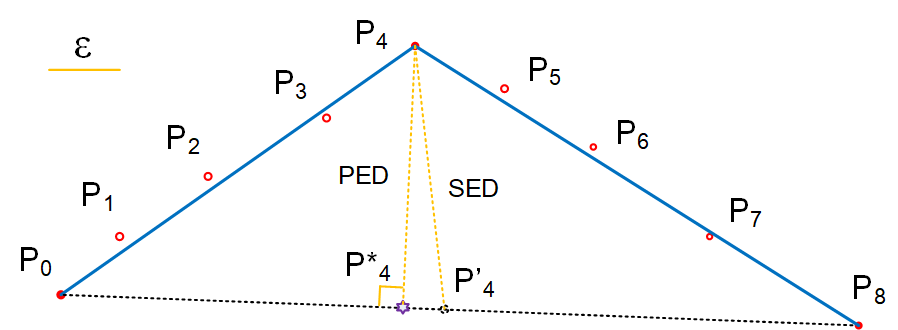
\includegraphics[scale=0.9]{Figures/Fig-Concepts.png}\vspace{-1ex}
	\caption{\small  A trajectory $\dddot{\mathcal{T}}[P_0, \ldots, P_{8}]$ with 9 points is simplified to (or represented by) two continuous line segments $ \overline{\mathcal{T}}[\overline{P_0P_4}, \overline{P_4P_{8}}] $ using \ped and \sed, respectively. In which, (1) $ped(P_4, \overline{P_0P_{8}})=|\overline{P_4P^*_4}|$, where $P^*_4$ is the perpendicular point of $P_4$ \wrt line segment $\overline{P_0P_{8}}$, and (2) $sed(P_4, \overline{P_0P_{8}})= |\overline{P_4P'_4}|$, where $P'_4$ is the synchronized point of $P_4$ \wrt $\overline{P_0P_{8}}$ satisfies ${|\overline{P_0P'_4}|}/{|\overline{P_0P_{8}}|} = \frac{(P_4.t - P_0.t)}{(P_{8}.t-P_0.t)} = \frac{(4-0)}{(8-0)}= \frac{1}{2}$.}
	\vspace{-2ex}
	\label{fig:concepts}
\end{figure}


\subsection{Notations}


%We first introduce basic notations.
\stitle{Trajectory}. A \textit{trajectory} $\dddot{\mathcal{T}}\left[P_0, \ldots, P_n\right]$ is a sequence of points in a monotonically increasing order of their associated time values (\ie $P_i.t < P_j.t$ for any $0\le i<j\le n$), where a data \textit{point} is defined as a triple $P\left(x, y, t\right)$, which represents that a moving object is located at {\em longitude} $x$ and {\em latitude} $y$ at {\em time} $t$. 
%Note that data points can be viewed as points in a three-dimension Euclidean space.


\eat{
	A \textit{line segment} (or line segment for simplicity) $\mathcal{L}$ is defined as $\overline{P_{s}P_{e}}$, which represents the closed line segment that connects the start point $P_s$ and the end point $P_e$.
	We also use $|\mathcal{L}|$ and $\mathcal{L}.\theta\in [0, 2\pi)$ to denote the length of a line segment $\mathcal{L}$, and its angle with the $x$-axis of the coordinate system $(x, y)$, where $x$ and $y$ are the longitude and latitude, respectively.
	That is, a line segment $\mathcal{L}$ = $\overline{P_{s}P_{e}}$ can be treated as a triple $(P_s, |\mathcal{L}|, \mathcal{L}.\theta)$.
}

%Intuitively, a trajectory can also be represented by a continuous $n$-pieces line segments (or line segment for simplicity) $\mathcal{L}_i$, $0\le i < n$, where  $\mathcal{L}_i = \overline{P_{i}P_{i+1}}$, represents the closed line segment that connects the start point $P_{i}$ and the end point $P_{i+1}$.

\stitle{Piece-wise line representation}. A \textit{piece-wise line representation} $\overline{\mathcal{T}}\left[\mathcal{L}_0, \ldots, \mathcal{L}_m\right]$ ($0< m \le n$) of a trajectory $\dddot{\mathcal{T}}\left[P_0, \ldots, P_n\right]$ is a sequence of continuous \textit{line segments} $\mathcal{L}_{i}$ = $\overline{P_{s_i}P_{e_i}}$ ($i\in\left[0,m\right]$) of $\dddot{\mathcal{T}}$ such that $\mathcal{L}_{0}.P_{s_0} = P_0$, $\mathcal{L}_{m}.P_{e_m} = P_n$ and  $\mathcal{L}_{i}.P_{e_i}$ = $\mathcal{L}_{i+1}.P_{s_{i+1}}$ for all $i\in\left[0, m-1\right]$.
Note that each line segment in $\overline{\mathcal{T}}$ essentially represents a continuous sequence of data points in trajectory $\dddot{\mathcal{T}}$.



For trajectory simplification, two Euclidean distance metrics are commonly used, namely, the \emph{perpendicular Euclidean distance} (\ped) and the \emph{synchronous Euclidean distance} \cite{Meratnia:Spatiotemporal} (\sed). Among them, \sed is also used in position and trajectory tracking.
%
Consider a data point $P$ and a line segment $\mathcal{L}$ = $\overline{P_{s}P_{e}}$.

\stitle{Perpendicular Euclidean distance}. The perpendicular Euclidean distance $ped\left(P, \mathcal{L}\right)$ of point $P$ to line segment $\mathcal{L}$ is $\min\{|PQ|\}$ for any point $Q$ on $\overline{P_{s}P_{e}}$.

\stitle{Synchronous Euclidean distance}. The synchronous Euclidean distance $sed\left(P, \mathcal{L}\right)$ of point $P$ to line segment $\mathcal{L}$ is $|\overline{PP'}|$ that is the Euclidean distance from $P$ to its \textit{synchronized point} $P'$ \wrt $\mathcal{L}$, where the synchronized point $P'$ \wrt $\mathcal{L}$ is defined as follows:
(a) $P'.x$ = $P_s.x +  c\cdot\left(P_e.x - P_s.x\right)$,
(b) $P'.y$ = $P_s.y +  c\cdot\left(P_e.y - P_s.y\right)$ and
(c) $P'.t$ = $P.t$, where $c= \frac{P.t-P_s.t}{P_e.t-P_s.t}$.

The \emph{synchronized point} $P'$ of a point $P$ \wrt line segment $\overline{P_sP_e}$ is the expected position of the moving object on $\overline{P_sP_e}$ at time $P.t$, obtained by a linear interpolation \cite{Cao:Spatio} that assumes it moved along the straight line from $P_s$ to $P_e$ with a uniform speed of $\frac{|\overline{P_sP_e}|}{P_e.t-P_s.t}$.


%Synchronized points are essentially virtual points with the assumption that an object moved along a straight line from $P_s$ to $P_e$ with a uniform speed, \ie the average speed $\frac{|\overline{P_sP_e}|}{P_e.t-P_s.t}$ between points $P_s$ and $P_e$ \cite{Cao:Spatio,Lin:Cised}. 

%More specifically, a synchronized point $P'_i$ of $P_i$ ($s\le i < e$) \wrt the line segment $\overline{P_sP_e}$ is a point on $\overline{P_sP_{e}}$ satisfying ${|\overline{P_sP'_i}|} = \frac{P_i.t - P_s.t}{P_e.t - P_s.t}\cdot {|\overline{P_sP_e}|}$, which means that the object moves from $P_s$ to $P_e$ at an average speed $\frac{|\overline{P_sP_e}|}{P_e.t-P_s.t}$, and its position at time $P_i.t$ is the point $P'_i$ on $\overrightarrow{P_sP_{e}}$ having a distance of $\frac{P_i.t - P_s.t}{P_e.t - P_s.t}\cdot|\overline{P_sP_e}|$ to $P_s$~\cite{Cao:Spatio, Lin:Cised,Meratnia:Spatiotemporal, Chen:Fast, Zhang:Evaluation}.


We illustrate these notations with examples shown in {Figure}~\ref{fig:concepts}.



 
 


\eat{%%%%%%%%%%%%%%
\begin{example}
	\label{exm-notations}
	Consider {Figure}~\ref{fig:concepts}, in which
	%
	(1) $\dddot{\mathcal{T}}\left[P_0, \ldots, P_{8}\right]$ is a trajectory having 9 data points,
	%
	(2) a set of two continuous line segments $\{\overline{P_0P_4}$, $\overline{P_4P_{8}}$\} is a piece-wise line representation of trajectory $\dddot{\mathcal{T}}$,
	%
	(3) $ped\left(P_4, \overline{P_0P_{8}}\right)=|\overline{P_4P^*_4}|$, where $P^*_4$ is the perpendicular point of $P_4$ \wrt line segment $\overline{P_0P_{8}}$, and 
	%
	(4) $sed\left(P_4, \overline{P_0P_{8}}\right)= |\overline{P_4P'_4}|$,
	where $P'_4$ is the synchronized point of $P_4$ \wrt $\overline{P_0P_{8}}$ satisfies $\frac{|\overline{P_0P'_4}|}{|\overline{P_0P_{8}}|} = \frac{P_4.t - P_0.t}{P_{8}.t-P_0.t} = \frac{4-0}{8-0}= \frac{1}{2}$.
\end{example}
}%%%%%%%%%%%%eat

\eat{%%%%%%%%%%%%%%%%%%
\stitle{Direction-aware distance distance}.The direction-aware distance $dad\left(\mathcal{L}_1, \mathcal{L}_2\right)$ is the direction deviation from $\mathcal{L}_1$ to $\mathcal{L}_2$, \ie $\Delta\left(\mathcal{L}_1.\theta, \mathcal{L}_2.\theta\right) = \min\{|\mathcal{L}_1.\theta - \mathcal{L}_2.\theta|, 2\pi - |\mathcal{L}_1.\theta - \mathcal{L}_2.\theta|\}$, where $\theta \in \left[0, 2\pi\right)$ is the angular of $\mathcal{L}$.
\textcolor{blue}{Note \dad differs from \ped and \sed in that it is a measure of angle, rather than Euclidean distances, and the temporal information is also lost when using \dad.}

\stitle{Trajectory simplification (Min-$\#$ problem).}
Given a trajectory \trajec{T}$\left[P_0, \dots, P_n\right]$ and a pre-specified constant $\epsilon$, the \emph{min-$\#$} problem of trajectory simplification is to approximate the trajectory \trajec{T} with $\overline{\mathcal{T}}\left[\mathcal{L}_0, \ldots , \mathcal{L}_m\right]$ ($0< m \le n$), such that
(1) on each of them the points $\left[P_{s_i}, \dots, P_{e_i}\right]$ are approximated by a line segment $\mathcal{L}_i = \overline{P_{s_i}P_{e_i}}$ with the maximum \ped or \sed \emph{error} of point $P_j$ (or \dad \emph{error} of line segment $|\overline{P_jP_{j+1}}|$) to line segment $\mathcal{L}_i$, $s_i \le j<e_i$,  less than $\epsilon$, and
(2) $P_{s_i}$ and $P_{e_i} \in$ \trajec{T}.


\stitle{Position tracking}. \textcolor{blue}{Given an error bound $\epsilon$, the position tracking is an agreement between a moving object and a MOD server such that the MOD server can infer the current position of the object with an deviation less than $\epsilon$ to its actual position.}

\stitle{Trajectory tracking}. It is a method implementing both trajectory simplification and position tracking.
}%%%%%%%%%%End EAT

\subsection{Position tracking in a circular area}

\textit{Position tracking} aims at informing the MOD about the current position of an object. Currently, the most simple yet efficient position tracking protocols is linear dead reckoning (\ldr) \cite{ Wolfson:PositionTracking}, which is essentially an agreement between a given moving object and the MOD server whose purpose is to let the MOD server track a moving object with less communication between them at an expense of imprecise of position within an error bound $\epsilon$.  

Given an error bound $\epsilon$, the moving object sends its initial location $P_s$ and the expected velocity $\vv{v}$
(including value and direction) to the MOD server, meaning that it is supposed to move from $P_s$ along the direction of $\vv{v}$ at a speed of $|\vv{v}|$, such that the expected position (\ie synchronized point) of the object at time $t>t_s$ can be extrapolated from them as long as no subsequent update is sent to the MOD server. 
After that, because the actual speed of it may be varied and different from the supposed speed of $|\vv{v}|$, the moving object periodically collects its actual position by sampling its on-board sensor, \eg GPS, and compares the actual position of time $t$ with the expected position of time $t$ extrapolated from the initial position $P_s$ and the velocity $\vv{v}$. 
If the deviation from its actual position to the expected position (\ie the synchronous Euclidean distance) is not more than $\epsilon$, then the object does not transmit any new updates to MOD, otherwise, an update of new ($P_s$, $\vv{v}$) will be sent.
%
By this way, though the MOD server receives less position information about a moving object, it still knows the expected position of the moving object with a bounded error of $\epsilon$ to its actual position. The \ldr mechanism ensures that no message is sent as long as the actual position $P$ is in the circular area around the excepted position $P'$ with a radius of $\epsilon$. That is, \emph{\ldr tracks a moving object in a floating circle having a velocity of $\vv{v}$.}

\begin{figure}[tb!]
	\centering
	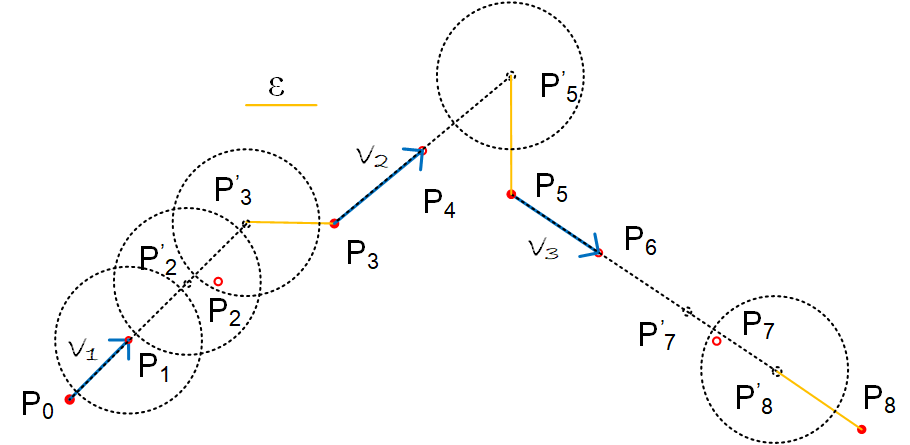
\includegraphics[scale=0.9]{figures/Fig-LDR.png}
	\vspace{-1ex}
	\caption{\small A running example of position tracking by \ldr. }
	\vspace{-1.5ex}
	\label{fig:ldr}
\end{figure}

\begin{example}
	\label{exm-ldr}
Figure \ref{fig:ldr} is a running example of \ldr.
Initially, point $P_0$ is set as $P_s$ and $\vec{v}$ is set to $\vec{v}_0$. Then, (1) points $P_1$ and $P_2$ have \sed distances less than $\epsilon$ to their expected points $P'_1$ and $P'_2$, respectively, and (2) $|P_3P'_3| > \epsilon$, meaning $P_3$ breaks the distance threshold, thus, a new update is triggered and $P_3$ is the new start point of the next section of position tracking.
%
\end{example}

%This example also demonstrates that (1) the expected position is indeed the synchronized point of the moving object at time $t$, (2) the deviation from the actual position to the expected position \wrt $\vv{v}$ is sure the synchronous Euclidean distance (\sed), and (3) 

 




\subsection{Trajectory tracking in a circular area}
\textit{Trajectory tracking} aims to implement both position tracking and trajectory simplification in one routine \cite{Lange:Tracking}. Currently, the one-pass trajectory tracking algorithm is a variation of \ldr, originally developed in \cite{Trajcevski:LDRH} and formally named as linear dead reckoning with half $\epsilon$ (\ldrh) in \cite{Lange:Tracking}.
%
Authors in \cite{Trajcevski:LDRH} proved that \ldr with some small variations is also a line simplification algorithm. Thus, \ldrh supports both position tracking and trajectory simplification, meaning it is a trajectory tracking algorithm.

Given an error bound $\epsilon$, \ldrh runs the same routine as \ldr except that (1) it uses half $\epsilon$ as the threshold in distance checking; (2) when the current point $P_k$ has a \sed larger than $\epsilon/2$ to its expected location (synchronous data point), it sends the preview point $P_{k-1}$ and a new $\vv{v}$ to the MOD server and continues trajectory tracking taking $P_{k-1}$ as the new start point. \ldrh is simple and efficient, having a linear time and a constant space. However, it has a poor effectiveness in terms of compression ratio, as the half $\epsilon$ is conservative, and more important, the algorithm is sensitive to the initial velocity which is set at the updating time but it is hard to be appropriate when the process goes on.

\begin{example}
Figure~\ref{fig:ldrh} is a running example of \ldrh taking the same input as Figure \ref{fig:ldr}.
Initially, the start point $P_s$ is set to $P_0$ and the velocity $\vec{v}$ is set to $\vec{v}_0$. Then, (1) $P_1$ and $P_2$ have \sed distances less than $\epsilon/2$ to their expected points $P'_1$ and $P'_2$, respectively, (2) $|P_3P'_3| > \epsilon/2$, thus, a new update is triggered and $P_2$ is the new start point of the next section of trajectory tracking. Finally, this algorithm in turn sends 5 points, $P_0, P_2, P_4, P_6$ and $P_8$, and 4 velocities, $\vec{v_1}$, $\vec{v_2}$, $\vec{v_3}$ and $\vec{v_4}$, to the MOD server.
\end{example}

\begin{figure}[tb!]
	\centering
	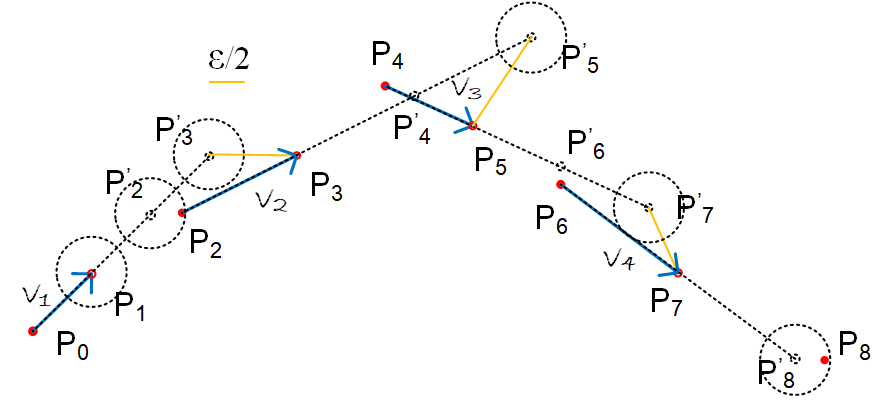
\includegraphics[scale=1.0]{figures/Fig-LDRH.png}
	\vspace{-1.5ex}
	\caption{\small A running example of trajectory tracking by \ldrh. }
	\vspace{-2ex}
	\label{fig:ldrh}
\end{figure}

%%%%%%
\eat{ 
	\textcolor{blue}{ 
		Lange et al. in \cite{Lange:GRTS, Lange:Tracking} introduced \grts framework that aimed at improving the effectiveness, in terms of compression ratio, of trajectory tracking by logically separating position tracking and trajectory simplification into two sub-processes, where position tracking is implemented by \ldr and trajectory simplification is enforced by integrating the third party line simplification algorithms \cite{Zhang:Evaluation, Lin:Cised}. \grts is effective than \ldrh, however, it is much more complex as it includes two sub-processes and introduces a buffer to temporarily save data points for the purpose of compression.
		Like \ldr, algorithms \ldrh and \grts both use \sed to check distances, hence, they also track a moving object in a floating circular area.}
}
%%%%%%eat







\subsection{Trajectory simplification based on spatio-temporal cones}

The recent trajectory simplification algorithm using \sed, namely \cised \cite{Lin:Cised}, is one-pass and also has a good effectiveness in terms of compression ratios. \cised uses a local synchronous distance checking approach based on a concept of \textit{spatio-temporal cone}, defined in a 3D Cartesian coordinate system whose $x$-axis, $y$-axis and $t$-axis are longitude, latitude and time, respectively, that converts the \sed distance tolerance into cones intersection for testing the successive points. This mechanism is potential to be extended for trajectory tracking with good effectiveness and efficiency.

\stitle{Spatio-temporal cone (\cone{}) \cite{Lin:Cised}}. 
Given a start point $P_s$ of sub-trajectory $\dddot{\mathcal{T}}_s[P_s, \ldots, P_{s+k}]$ and an error bound $\epsilon$, the spatio-temporal cone (or simply \textit{cone}) of a data point $P_{s+i}$ ($1\le i\le k$) in $\dddot{\mathcal{T}_s}$ \wrt $P_s$ and $\epsilon$, denoted as \cone{(P_s, P_{s+i}, \epsilon)}, or \cone{_{s+i}} in short, is an oblique circular cone such that point $P_s$ is its apex and the synchronous circle $\mathcal{O}(P_{s+i}, \epsilon)$ of point $P_{s+i}$, or \circle{_{s+i}} in short, a circle on the plane $P.t-P_{s+i}.t = 0$ such that $P_{s+i}$ is its center and $\epsilon$ is its radius, is its base (Figure~\ref{fig:cis}).

\eat{%%%%%%%%%%%
	\begin{example}
		\label{exm-circles-cones}
		Figure~\ref{fig:cis} shows 
		(1) two synchronous circles, \circle{(P_{s+i}, \epsilon)} of point $P_{s+i}$ and \circle{(P_{s+k}, \epsilon)} of point $P_{s+k}$.
		It is easy to see that for any point in the area of a circle \circle{(P_{s+i}, \epsilon)}, its distance to $P_{s+i}$ is not greater than $\epsilon$, 
		and (2) two example spatio-temporal cones, \cone{(P_s, P_{s+i}, \epsilon)} {(purple)} and \cone{(P_s, P_{s+k}, \epsilon)} (red), with the same apex $P_s$ and error bound $\epsilon$. %\eop
	\end{example}
}%%%%%%%%%%%

%Note that in this definition, a \emph{synchronous circle} $\mathcal{O}(P_i, \epsilon)$ is only defined by a central point $P_i$ and a constant $\epsilon$. Indeed, it is nothing to do with any start point $P_s$ or end point $P_e$.


%\textcolor{blue}{We define \textit{synchronous circles and Spatio-temporal cones} in a \emph{x-y-t} 3D coordinate system, and build the connection between \textit{synchronous circles} and \textit{synchronous distances}.}



\begin{figure}[tb!]
	\centering
	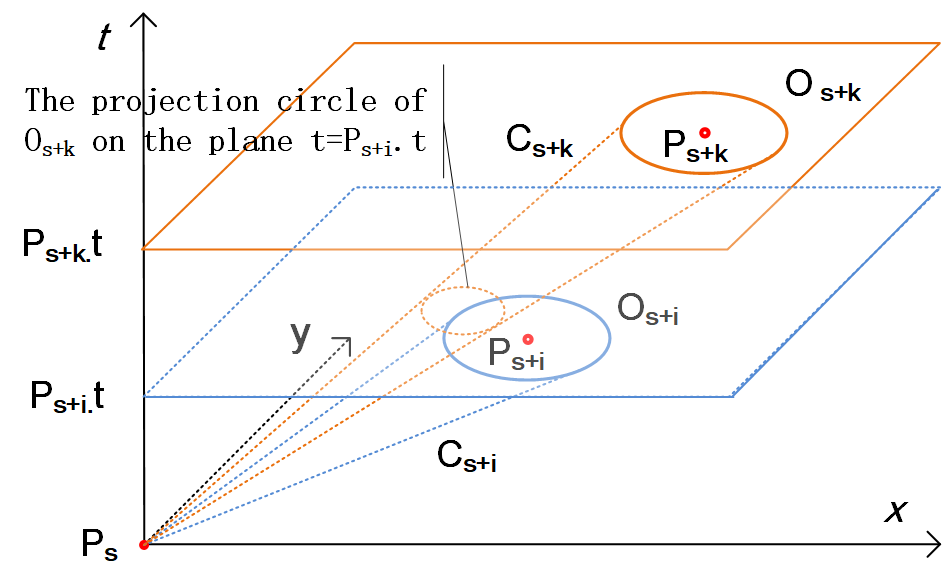
\includegraphics[scale=0.88]{figures/Fig-CIS.png}
	\vspace{-2ex}
	\caption{\small Examples of spatio-temporal cones in a 3D Cartesian coordinate system taking point $P_s$ as the origin, where (1) $P_{s+i}$ and $P_{s+k}$ are two points, (2) \circle{_{s+i}} and \circle{_{s+k}} are two synchronous circles, (3) \cone{_{s+i}} and \cone{_{s+k}} are two spatio-temporal cones.}
	\vspace{-1ex}
	\label{fig:cis}
\end{figure}
%, (4) $Q$ is a point in synchronous circle \circle{_{s+k}}, and (5) $P'_{s+i}$ is the intersection point of line $\protect\overline{P_sQ}$ and synchronous circle \circle{_{s+i}}

Based on the spatio-temporal cone, authors in \cite{Lin:Cised} prove that the \sed distance tolerance can be checked by finding the common intersection of spatio-temporal cones  (half-$\epsilon$) built from points of a sub-trajectory $[P_s,...,P_{s+k}]$, \ie ``{given a sub-trajectory $[P_s,...,P_{s+k}]$ and an error bound $\epsilon$, $sed(P_{s+i}, \overline{P_sP_{s+k}})\le \epsilon$ for each $i \in [1,k]$ if  $\bigsqcap_{i=1}^{k}$\cone{(P_s, P_{s+i}, \epsilon/2)} $\ne \{P_s\}$}."
In other words, if these cones do have a common intersection, then line segment $\overline{P_sP_{s+k}}$ can represent the sub-trajectory. And for efficiency consideration, \cised projects those cones on a plane, \eg plane $t=P_{s+1}.t$, so as to convert the checking of cones intersection into a much simpler way, \ie~\textit{checking of circles intersection on the plane} (Figure~\ref{fig:cis}).
For the same reason, a circle is further approximated by its inscribe regular polygon and the intersecting of circles is approximated by the intersecting of these polygons, which can be computed in linear time.
%
%Note that though the cone intersection approach outperform the counterpart of \ldr and \ldrh, it is still not introduced to trajectory tracking.

\eat{%%%%%%%%%%%%%%%%%% Delete because of the page limitation.
	Figure~\ref{fig:cised} is a running example of \cised. In this case, it outperforms \ldrh in terms of compression ratio.
	
	\begin{figure}[tb!]
		\centering
		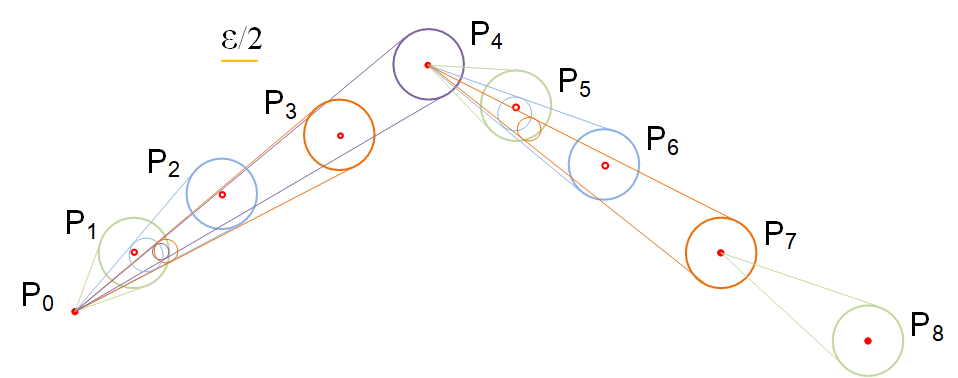
\includegraphics[scale=0.9]{figures/Fig-CISED-SH.png}
		\vspace{-1ex}
		\caption{\small A running example of \cised. In the first section, cones are projected on plane $P_1.t$, where (1) the projection circles of \circle{_{1}},\circle{_{2}},\circle{_{3}} and \circle{_{4}} have common intersection, and (2) it does not intersected with the projection circle of \circle{_{5}}. Thus, $P_4$ is output, and it serves as the new start point of the next section. Finally, the same trajectory is simplified to four points $\{P_0, P_4, P_7, P_8\}$.}
		\vspace{-2ex}
		\label{fig:cised}
	\end{figure}
}%%%%%%%%%%%%%%%%%%%%%%



%\subsection{Trajectory simplification in strip areas}
%\todo{sleeve (half-epsilon)}

